%=====================================================
% PREÂMBULO - CONFIGURAÇÕES GERAIS DO DOCUMENTO
%======================================================
\documentclass[12pt, a4paper, openright, oneside, brazilian]{abntex2}

% --- PACOTES DE CODIFICAÇÃO ---
\usepackage{fontenc}
\usepackage[utf8]{inputenc}

% --- PACOTES DE LAYOUT E FORMATAÇÃO (ABNT/UNESP) ---
\usepackage[left=3cm, top=3cm, right=2cm, bottom=2cm, headsep=1.5cm]{geometry}
\usepackage{indentfirst} % Indenta o primeiro parágrafo de cada seção
% Usando o comando nativo da classe memoir (base do abntex2) para espaçamento 1,5 [1]
\OnehalfSpacing
% --- PACOTES DE BIBLIOGRAFIA (ABNT) ---
\usepackage{csquotes}
% Opções simplificadas para máxima compatibilidade.
\usepackage[backend=biber, style=abnt]{biblatex}
\addbibresource{bibliografia.bib} % Seu arquivo.bib

% --- PACOTES MATEMÁTICOS ---
\usepackage{amsmath}
\usepackage{amssymb}
\usepackage{mathtools}

% --- PACOTES PARA TABELAS E FIGURAS ---
\usepackage{graphicx}
\usepackage{booktabs}
\usepackage{multirow}
\usepackage{array}
\usepackage[table]{xcolor}
\usepackage{caption}
\usepackage{float}
\captionsetup{
    format=plain,
    justification=justified,
    singlelinecheck=false,
    font=small,
    labelfont=bf,
    labelsep=period
}

% --- PACOTES ADICIONAIS ---
\usepackage{ragged2e}
\usepackage{soul}

% --- CONFIGURAÇÃO DE HIPERLINKS ---
\hypersetup{
    colorlinks=true,
    linkcolor=black,
    citecolor=black,
    urlcolor=black,
    pdftitle={Desenvolvimento e Análise de um Controlador Eletrônico de Velocidade para Motores de Corrente Contínua Sem Escovas},
    pdfauthor={Enzo Luiz Fernandes},
    bookmarksopen=true
}

%=====================================================
% METADADOS DO TRABALHO (PARA CAPA E FOLHA DE ROSTO AUTOMÁTICAS)
%=====================================================

\titulo{Desenvolvimento e Análise de um Controlador Eletrônico de Velocidade para Motores de Corrente Contínua Sem Escovas}
\autor{Enzo Luiz Fernandes}
\instituicao{
  Universidade Estadual Paulista "Júlio de Mesquita Filho"
  \par
  Faculdade de Engenharia de Ilha Solteira
  \par
  Departamento de Engenharia Elétrica
}
\local{Ilha Solteira}
\data{2025}
\tipotrabalho{Trabalho de Conclusão de Curso}
\orientador{Prof. Dr. Guilherme de Azevedo e Melo}
\tipotrabalho{monografia}
\preambulo{Trabalho de Conclusão de Curso apresentado ao Departamento de Engenharia Elétrica da Faculdade de Engenharia de Ilha Solteira, da Universidade Estadual Paulista "Júlio de Mesquita Filho", como parte dos requisitos para obtenção do título de Bacharel em Engenharia Elétrica.}

\begin{document}

% --- ELEMENTOS PRÉ-TEXTUAIS --
\begin{center}

\includegraphics[width=9cm]{imagens/logoUNESP.jpg} 
\end{center}

\vspace{1.5cm} 
\imprimircapa
%\imprimirfolhaderosto

% Folha de Aprovação
\begin{folhadeaprovacao} 
\begin{center}
{\ABNTEXchapterfont\large\textsc{\imprimirautor}}
\par\vspace{\onelineskip}
{\ABNTEXchapterfont\Large\bfseries\imprimirtitulo} 
\end{center} 
\vspace{1cm} 
\hspace{.45\textwidth} \begin{minipage}{.5\textwidth} 
\imprimirpreambulo 
\end{minipage} 
\vspace{1cm}
\par\vspace{\onelineskip}
Trabalho aprovado. \imprimirlocal, \imprimirdata: 

%Assinaturas 
\assinatura{\imprimirorientador \\UNESP} 
\assinatura{Assinatura 2\\ UNESP} 
\assinatura{Assinatura 3 \\ UNESP} 

\begin{center} 
\vfill 
{\large\imprimirlocal} 
\par 
{\large\imprimirdata} 
\end{center} 
\end{folhadeaprovacao}

% RESUMO E ABSTRACT
\begin{abstract}
    Este trabalho aborda o desenvolvimento e a análise de um controlador eletrônico de velocidade (ESC) para motores de corrente contínua sem escovas (BLDC). A investigação inicia com uma robusta fundamentação teórica sobre os princípios de funcionamento, construção e os parâmetros chave dos motores BLDC, como as constantes de torque ($K_T$) e de velocidade ($K_V$), cuja equivalência intrínseca é demonstrada por meio de um balanço de potência. Em seguida, são detalhados os algoritmos de controle, com foco na comutação de seis passos e na modulação por largura de pulso (PWM). A metodologia do projeto é delineada em três fases: simulação computacional para validação do conceito, projeto do circuito eletrônico com seleção criteriosa de componentes incluindo o microcontrolador ESP32 e uma bateria LiPo dimensionada para a aplicação e, por fim, a prototipagem e testes experimentais para verificar o desempenho do controlador. O objetivo é produzir um protótipo funcional que ofereça uma operação suave e precisa, validando os conceitos teóricos e as escolhas de projeto.
    \par\vspace{\onelineskip} % Espaço antes das palavras-chave
    \noindent\textbf{Palavras-chave:} Motor BLDC. Controlador Eletrônico de Velocidade. Controle de Motores. ESP32.
\end{abstract}

\begin{abstract} 
\begin{otherlanguage*}{english}
This work addresses the development and analysis of an electronic speed controller (ESC) for brushless direct current (BLDC) motors. The investigation begins with a robust theoretical foundation on the operating principles, construction, and key parameters of BLDC motors, such as the torque ($K_T$) and velocity ($K_V$) constants, whose intrinsic equivalence is demonstrated through a power balance analysis. Subsequently, control algorithms are detailed, focusing on six-step commutation and pulse-width modulation (PWM). The project methodology is outlined in three phases: computational simulation for concept validation, electronic circuit design with careful selection of components—including the ESP32 microcontroller and a LiPo battery sized for the application—and finally, prototyping and experimental testing to verify the controller's performance. The objective is to produce a functional prototype that offers smooth and precise operation, validating the theoretical concepts and design choices.
    \par\vspace{\onelineskip}
    \noindent\textbf{Keywords:} BLDC Motor. Electronic Speed Controller. Motor Control. ESP32.
\end{otherlanguage*}
\end{abstract}

% LISTAS E SUMÁRIO

\newpage
\pdfbookmark{\listfigurename}{lof}
\listoffigures*
\cleardoublepage

\pdfbookmark{\listtablename}{lot}
\listoftables*
\cleardoublepage

\pdfbookmark{\contentsname}{toc}
\tableofcontents*
\cleardoublepage

% --- ELEMENTOS TEXTUAIS ---
\textual

\chapter{Introdução Teórica}

Os motores BLDC (\textit{Brushless Direct Current Motor}) representam um avanço significativo em relação aos motores CC tradicionais porque eliminam a necessidade de escovas mecânicas para a conversão de energia, resultando em maior rendimento energético, menos desgaste e maior vida útil \cite{hanselman2003brushless}. Esses avanços tecnológicos estão sendo impulsionados pela crescente demanda por sistemas de acionamento mais eficientes, confiáveis e de baixa manutenção em diversas aplicações industriais, comerciais e de consumo. A precisão e controlabilidade dos motores BLDC os tornam ideais para aplicações que exigem alta exatidão de movimento, velocidade e controle de torque, como robótica, automação industrial, veículos elétricos e eletrônicos de consumo.

\section{Motores CC Sem Escova}
O princípio de funcionamento dos motores BLDC é baseado em campos magnéticos gerados por ímãs permanentes e enrolamentos de  (Figura \ref{Configuração de um motor DC convencional (A) e motor BLDC (B).}). A comutação da corrente para gerar movimento ocorre eletronicamente, por meio de um controlador dedicado normalmente chamado de ESC (Eletronic Speed Controller), que pode usar ou não sensores durante o processo, eliminando assim a necessidade de escovas mecânicas utilizadas em motores DC tradicionais. Esta abordagem resulta em uma diminuição significativa do desgaste mecânico, aumentando a vida útil do motor e reduzindo a necessidade de manutenção.

\begin{figure}[h]
	\centering
	\caption{Configuração de um motor DC convencional (A) e motor BLDC (B).}
	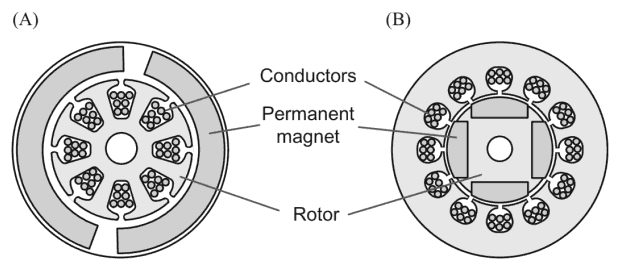
\includegraphics[width=8cm]{imagens/Comparativo.png}
	\caption*{Fonte:\cite{kim2017electric}.}
 \label{Configuração de um motor DC convencional (A) e motor BLDC (B).}
\end{figure}

Amplamente utilizados em uma variedade de aplicações, desde eletrônicos de consumo, como ventiladores e ferramentas elétricas, até aplicações industriais e automotivas. Sua capacidade de fornecer um controle preciso de velocidade e posição, juntamente com uma resposta rápida, faz deles a escolha ideal para sistemas que exigem rendimento energético e alta performance.

Apesar das muitas vantagens, não estão isentos de algumas limitações. A complexidade eletrônica necessária para o controle preciso, o custo inicial potencialmente mais elevado comparado a motores elétricos escovados, a sensibilidade a ambientes de alta temperatura, pois podem gerar a desmagnetização dos imãs permanentes, a exigência de eletrônica de controle especializada, o potencial de ruído eletromagnético (EMI) e a complexidade de manutenção do sistema como um todo são fatores a serem considerados ao escolher essa tecnologia. Cada aplicação específica deve ponderar essas considerações em relação aos benefícios que os BLDC oferecem, como rendimento, durabilidade e controle superior.

São categorizados como síncronos, ou seja, o rotor gira na mesma frequência do campo magnético gerado pelo estator \cite{jahns1984torque}. Também não apresentam o fenômeno de escorregamento que é característico dos motores de indução. Os motores BLDC estão disponíveis em configurações de uma fase, duas fases e três fases, sendo  essa a mais amplamente utilizada, por serem equilibrados em relação a oscilação de torque e custo de construção \cite{hendershot1994design}.

A nomenclatura "Brushless DC" pode gerar uma interpretação equivocada. Embora alimentado por uma fonte de corrente contínua (DC), o motor BLDC é, em sua essência, um motor síncrono de ímãs permanentes (PMSM) \parencite{maquinasEletricasFitzgerald}. A rotação é induzida por campos magnéticos girantes gerados nos enrolamentos do estator, que são alimentados por formas de onda de corrente alternada (AC) sintetizadas por um controlador eletrônico. Portanto, a designação "DC" refere-se à fonte de alimentação externa, e não ao princípio físico de operação interna, que requer uma lógica de controle sofisticada para operar \parencite{ti2013sensorless}.

Nesse contexto, a performance do sistema é governada por parâmetros intrínsecos que descrevem a física da conversão de energia. Duas das mais importantes dessas constantes são a \textbf{constante de torque ($K_T$)} e a \textbf{constante de velocidade ($K_V$)}. Estes parâmetros são a manifestação matemática dos princípios físicos que regem a interação entre os domínios elétrico e mecânico do motor.

\subsection{Fundamentos Físicos da Conversão Eletromecânica}

A operação de um motor elétrico é governada por dois princípios físicos interligados: a Força de Lorentz, que gera o torque, e a Lei da Indução de Faraday, que gera uma força contraeletromotriz.

\subsubsection{A Força de Lorentz e a Condição de Torque Máximo}

A produção de força mecânica em um motor origina-se na Força de Lorentz. Esta lei descreve a força ($\vec{F}$) sobre um condutor de comprimento vetorial ($\vec{L}$) percorrido por uma corrente ($I$) e imerso em um campo magnético ($\vec{B}$). A relação vetorial é:
\begin{equation}
    \vec{F} = I(\vec{L} \times \vec{B})
\end{equation}
A magnitude desta força, $F = I L B \sin(\theta)$, onde $\theta$ é o ângulo entre o condutor e o campo magnético, é maximizada quando $\sin(\theta) = 1$, o que ocorre precisamente quando $\theta = 90^{\circ}$. Esta condição de ortogonalidade é o princípio mais elementar para a máxima conversão de energia.

Em um motor rotativo, o objetivo é o torque, que pode ser entendido como a interação entre o campo magnético gerado pelo estator ($\vec{B}_{\text{estator}}$) e o campo gerado pelos ímãs permanentes do rotor ($\vec{B}_{\text{rotor}}$). O torque eletromagnético ($\vec{T}_{em}$) é o produto vetorial desses dois campos \cite{vas1998vector}:
\begin{equation}
    \vec{T}_{em} \propto \vec{B}_{\text{estator}} \times \vec{B}_{\text{rotor}}
\end{equation}
A magnitude do torque é, portanto, diretamente proporcional ao seno do ângulo elétrico ($\theta_e$) entre os dois vetores de campo. O torque máximo é alcançado quando este ângulo é mantido em 90 graus elétricos. Manter esta condição de ortogonalidade de forma contínua é o objetivo central das estratégias de controle de alto desempenho, como o Controle Orientado por Campo (FOC), pois garante não apenas o torque máximo para uma dada corrente, mas também a máxima eficiência na conversão eletromecânica.

\subsubsection{A Lei de Faraday}
Simultaneamente à produção de torque, um motor em rotação atua como um gerador. A Lei da Indução de Faraday afirma que a variação do fluxo magnético através de uma espira de fio induz uma força eletromotriz (FEM). Em um motor, o movimento dos ímãs do rotor em relação aos enrolamentos do estator induz uma tensão conhecida como \textbf{força contraeletromotriz (FCEM)}, ou \textit{back-EMF}.

De acordo com a Lei de Lenz, a polaridade desta tensão induzida ($e_a$) se opõe diretamente à tensão terminal ($V$) aplicada ao motor \parencite{infineon2011bldc}. A magnitude da FCEM é diretamente proporcional à velocidade angular ($\omega$) do motor, estabelecendo a ligação física entre o movimento mecânico (velocidade) e um fenômeno elétrico (tensão induzida).

\subsection{Modelo Matemático do Motor e a Definição das Constantes}

Os princípios de Lorentz e Faraday são sintetizados em um modelo matemático que descreve a dinâmica do motor.

\textbf{Equação Elétrica (Lei de Kirchhoff):}
\begin{equation}
    V = e_a + I_a R_a + L_a \frac{dI_a}{dt}
\end{equation}
Onde $V$ é a tensão aplicada, $e_a$ é a FCEM de Armadura, $I_a R_a$ é a queda de tensão resistiva de Armadura e $L_a \frac{dI_a}{dt}$ é a queda de tensão indutiva de Armadura \parencite{maquinasEletricasFitzgerald}. Vale ressaltar que Armadura é o termo técnico para o enrolamento em motores elétricos, onde a principal conversão de energia acontece.

\textbf{Equação Mecânica (2ª Lei de Newton para Rotação):}
\begin{equation}
    T_e = T_l + J \frac{d\omega}{dt} + B\omega
\end{equation}
Onde $T_e$ é o torque eletromagnético, $T_l$ é o torque de carga, $J\frac{d\omega}{dt}$ é o torque inercial e $B\omega$ é o torque de atrito viscoso \parencite{maquinasEletricasFitzgerald}.

Dentro deste modelo, as constantes do motor surgem como os fatores de proporcionalidade que conectam os domínios elétrico e mecânico.

\subsection{\texorpdfstring{A constante de Torque $K_T$}{A constante de Torque KT}}
\label{KT}
A constante de torque ($K_T$) define a capacidade de um motor de converter corrente elétrica em torque mecânico. É formalmente definida como a relação linear:
\begin{equation}
    T_e = K_T I_a
\end{equation}
O valor de $K_T$ não é arbitrário, mas determinado pelas características construtivas do motor \parencite{hendershot1994design}:
\begin{itemize}
    \item \textbf{Força do Campo Magnético ($B$):} Ímãs mais fortes (ex: Neodímio) resultam em um $K_T$ maior.
    \item \textbf{Configuração do Enrolamento:} É diretamente proporcional ao número de espiras ($N$) nos enrolamentos.
    \item \textbf{Geometria do Motor:} Dimensões como o comprimento e o raio do estator influenciam diretamente seu valor.
\end{itemize}
Para um dado torque de carga, um motor com $K_T$ maior demandará uma corrente menor, resultando em menores perdas por efeito Joule ($P = I^2 R$) e, portanto, maior eficiência.

\subsection{\texorpdfstring{As constantes de Velocidade $K_V$}{As constantes de Velocidade KV}}
\label{KV}

De forma análoga, a relação entre a FCEM e a velocidade é quantificada por constantes.
\begin{itemize}
    \item \textbf{Constante de FCEM ($K_e$):} É a constante física que relaciona a FCEM gerada ($e_a$) com a velocidade angular do motor ($\omega$):
    \begin{equation}
        e_a = K_e \omega
    \end{equation}
    Assim como $K_T$, $K_e$ (também denotado como $k_b$) depende do projeto físico do motor \parencite{zoltan2012understanding}.

    \item \textbf{Constante de Velocidade ($K_V$):} Muito mais comum em folhas de dados comerciais, $K_V$ é definida como a relação entre a velocidade do motor sem carga e a tensão aplicada, geralmente em unidades de \textbf{RPM/V}. A relação entre $K_V$ e $K_e$ é de simples inversão \parencite{infineon2011bldc}:
    \begin{equation}
        K_V = \frac{1}{K_e}
    \end{equation}
    A FCEM é o mecanismo que limita a velocidade máxima do motor. O motor acelera até que a FCEM ($e_a = K_e \omega$) se aproxime da tensão de alimentação ($V$), ponto no qual a corrente resultante é apenas suficiente para vencer o atrito.
\end{itemize}

\subsection{A Equivalência entre $K_T$ e $K_e$}

Um dos resultados mais notáveis na teoria de motores é a equivalência numérica entre $K_T$ e $K_e$ quando ambas são expressas em unidades do Sistema Internacional (SI): \textbf{Nm/A} para $K_T$ e \textbf{V·s/rad} para $K_e$.
\begin{equation}
    K_T \text{ [Nm/A]} = K_e \text{ [V·s/rad]}
\end{equation}
Esta equivalência não é uma coincidência, mas uma consequência da \textbf{lei da conservação de energia}.

\textbf{Demonstração por Balanço de Potência:}
\begin{enumerate}
    \item A potência elétrica convertida em potência mecânica ($P_{\text{conv}}$) é a parte da potência de entrada que não é perdida como calor nos enrolamentos.
    \
    \item Usando a equação elétrica ($V = e_a + I_a R_a$), substituímos $V$:
    \
    \item A potência mecânica de saída ($P_{\text{mec}}$) é o produto do torque e da velocidade angular:
    \
    \item Pela conservação de energia, $P_{\text{conv}} = P_{\text{mec}}$:
    \
    \item Agora, substituímos as definições de $K_e$ e $K_T$ ($e_a = K_e \omega$ e $T_e = K_T I_a$):
    \
    \item Para qualquer condição de operação não nula, podemos cancelar $\omega$ e $I_a$ de ambos os lados, provando que:
    \begin{equation}
        K_e = K_T
    \end{equation}
\end{enumerate}
Esta prova revela que o mesmo mecanismo de acoplamento eletromagnético que produz torque a partir da corrente (princípio motor, $K_T$) é o que gera tensão a partir do movimento (princípio gerador, $K_e$). Eles são duas manifestações do mesmo fenômeno físico \parencite{zoltan2012understanding, garcia1997modelagem}.

\subsection{Conversão de Unidades}

A elegância teórica é frequentemente obscurecida pelo uso de unidades inconsistentes na prática. A habilidade de converter valores de folhas de dados para o padrão SI é indispensável. A relação prática mais importante é entre $K_T$ e $K_V$:
\begin{equation}
    K_T \text{ [N·m/A]} = \frac{2\pi }{60 \: K_V \text{ [RPM/V]}}
\end{equation}
Esta fórmula é derivada diretamente da equivalência $K_T = K_e = 1/K_V$ após a conversão de RPM para rad/s \parencite{infineon2011bldc}. A tabela abaixo resume as conversões chave.

\begin{table}[h!]
\centering
\caption{Unidades de Constantes de Motor e Fatores de Conversão para o SI}
\label{tab:unidades}

\resizebox{\columnwidth}{!}{

\begin{tabular}{llll}
\toprule
\textbf{Parâmetro} & \textbf{Unidade SI} & \textbf{Unidades Comuns Não-SI} & \textbf{Fórmula de Conversão para SI} \\
\midrule
\textbf{Constante de Torque ($K_T$)} & N·m/A & oz-in/A & 1 oz-in/A = 0.00706155 N·m/A \\
 & & mN·m/A & 1 mN·m/A = 0.001 N·m/A \\
\addlinespace
\textbf{Constante de FCEM ($K_e$)} & V·s/rad & V/krpm & 1 V/krpm = 0.009549 V·s/rad \\
\addlinespace
\textbf{Constante de Velocidade ($K_V$)} & rad/(V·s) & RPM/V & 1 RPM/V = 0.10472 rad/(V·s) \\
\bottomrule
\end{tabular}
}
\caption*{Fonte:Elaborado pelo autor.}
\end{table}

\subsection{A Constante do Motor ($K_m$) como Figura de Mérito}

Uma constante mais fundamental para avaliar a qualidade do projeto de um motor é a \textbf{constante do motor ($K_m$)}:
\begin{equation}
    K_m = \frac{K_T}{\sqrt{R_a}}
\end{equation}
Sua unidade no SI é \textbf{N·m/$\sqrt{\text{W}}$}. $K_m$ representa a capacidade do motor de produzir torque por watt de potência dissipada como calor. Um $K_m$ mais alto indica um motor mais eficiente na conversão de energia. Notavelmente, $K_m$ é invariante a alterações no enrolamento para um mesmo tamanho de carcaça, tornando-se uma excelente figura de mérito para comparar a qualidade de diferentes projetos de motores \parencite{infineon2011bldc}.

\subsection{Influência da Temperatura}

Embora chamadas de "constantes", $K_T$ e $K_e$ são afetadas pela temperatura. O aquecimento do motor causa uma redução na força magnética dos ímãs permanentes. Como ambas as constantes são diretamente proporcionais à densidade de fluxo magnético, um motor operando em alta temperatura produzirá menos torque para a mesma corrente (menor $K_T$) e precisará girar mais rápido para gerar a mesma FCEM (menor $K_e$, consequentemente um $K_V$ ligeiramente maior), resultando em uma performance geral degradada.

\section{Controlador Eletrônico de Velocidade (ESC)} 
 Os controladores eletrônicos de velocidade, são dispositivos eletrônicos que controlam a velocidade e o torque de motores BLDC. São classificados pela sua corrente e tensão máxima de saída. São constituídos dos seguintes componentes básicos: 

 \begin{itemize} 
 \item Circuito de entrada: O circuito de entrada converte a tensão fornecida pela bateria em tensão que pode ser usada pelo circuito de controle utilizando PWM para gerar uma tensão média desejada que será fornecida ao motor. Também pode inverter a sequência de comutação das fases fazendo com que o sentido de rotação também seja invertido. 
 \item Circuito de controle: O circuito de controle é responsável por calcular a corrente que deve ser fornecida às bobinas do motor. Normalmente se utilizam de sinais com características de PWM como sinal de referência para definir a velocidade e sentido de rotação. 
 \item Circuito de saída: O circuito de saída fornece a corrente necessária às bobinas do motor. 
 \end{itemize} 

 Além desses componentes básicos, os ESCs para motor BLDC pode incluir os seguintes recursos, além dos já discutidos anteriormente: 

 \begin{itemize} 
 \item Filtro de ruído: O filtro de ruído é usado para reduzir o ruído elétrico que pode ser gerado pelo motor. 
 \item Proteção térmica: A proteção térmica é usada para proteger o motor de superaquecimento. 
 \item Proteção contra sobrecarga: O ESC pode desligar o motor se ele experimentar correntes superiores às nominais que representam riscos de deterioração das bobinas do motor. 
 \end{itemize} 

  As equações lineares de um motor DC só são diretamente aplicáveis a um motor BLDC devido à ação sofisticada do seu \textbf{Controlador Eletrônico de Velocidade (ESC)}. O ESC realiza a comutação eletrônica, energizando sequencialmente os enrolamentos do estator para criar um campo magnético giratório. Isso força a complexa máquina AC a se comportar como o motor DC idealizado, tornando as constantes $K_T$ e $K_e$ ferramentas de análise e projeto perfeitamente válidas \parencite{hendershot1994design}.

 \subsection{Consequências Práticas da Seleção de $K_V$} 

 A seleção de $K_V$ é uma decisão de projeto crítica que estabelece um compromisso fundamental: 
 \begin{itemize} 
 \item \textbf{Motores de Alto $K_V$:} Possuem menos espiras de fio mais grosso. Resultam em baixo $K_T$, baixa resistência e baixa indutância. Para produzir torque, exigem alta corrente, mas atingem altas velocidades. Ideais para aplicações de alta velocidade e baixo torque, como drones de corrida e fusos de usinagem \parencite{tmotor2019kv}. 
 \item \textbf{Motores de Baixo $K_V$:} Possuem mais espiras de fio mais fino. Resultam em alto $K_T$, alta resistência e alta indutância. Geram alto torque com baixas correntes, sendo mais eficientes para essa finalidade, mas com menor velocidade máxima. Ideais para aplicações de acionamento direto e alto torque, como drones de carga, guinchos e atuadores robóticos \parencite{byod2018kv}. 
 \end{itemize} 

 \subsection{Princípios de Operação} 

  O controlador do motor deve fornecer corrente e tensão adequadas às bobinas do estator do motor, a fim de controlar a velocidade e o torque do motor \cite{jahns1996pulsating}. O circuito básico que realiza esse papel é o de uma ponte inversora trifásica, onde o motor BLDC pode estar conectado em Estrela ou Delta. O controle do circuito de disparo dos transistores do inversor deve ser feito de forma que cada fase do estator seja percorrida por uma corrente com a forma de onda senoidal ou trapezoidal, voltadas respectively para alto rendimento e baixo custo. As formas de onda de cada uma das fases devem estar defasadas entre si, permitindo que o motor gire de forma contínua. 

 \subsubsection{Comutação de Seis Passos} 

 A comutação de seis passos demanda um sincronismo de disparo dos transistores, de modo que sempre dois deles estejam fechados, formando um circuito tal que a cada $60 ^\circ$ elétricos o par de fases percorridas pela corrente se alterne (Figura \ref{Sequência de acionamento para um BLDC trifásico}). Cada transistor permanece em condução durante $120 ^\circ$ elétricos. Vale ressaltar que os eventos de condução e bloqueio, denominados comutações dos transistores, geram variações na corrente e isso é responsável pelas oscilações no torque do motor \cite{kim2017electric}.  

 \begin{figure}[p] 
     \centering 
     \caption{Sequência de acionamento para um BLDC trifásico.} 
     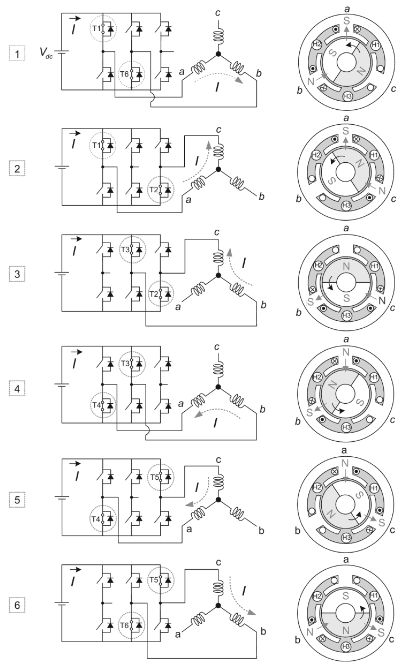
\includegraphics[width=10cm]{imagens/acionamento.png} 
     \caption*{Fonte:\cite{kim2017electric}.} 
  \label{Sequência de acionamento para um BLDC trifásico} 
 \end{figure} 

 Esse algoritmo de acionamento dos transistores, também chamado de Controle Trapezoidal, é um dos métodos utilizados para controlar motores BLDC. Para se saber quando e quais deles acionar, existem duas opções: o Controle de Malha Fechada, no qual é preciso saber a posição que o rotor se encontra de forma a acionar o conjunto de transistores seguinte, e o Controle de Malha Aberta. Neste último, é possível acionar os indutores a partir de uma sequência fixa determinada pelo circuito, o que faz com que o rotor comece a girar em algum momento da sequência e siga girando a partir da sequência determinada. Esse tipo de controle é mais simples e de menor custo, porém não tão preciso, recebendo o nome de Controle de Malha Aberta, e será o método inicialmente utilizado neste trabalho. 

  Para a realização do Controle de Malha Fechada é possível usar um sensor de efeito Hall capaz de identificar o campo magnético resultante da interação do campo eletromagnético das bobinas e do campo magnético dos imãs permanentes do rotor, indicando a seção que o campo eletromagnético resultante encontra-se, ou seja, sua posição angular. Partindo dessa referência, se pode saber quais transistores devem ser acionadas para que o rotor continue a girar. A utilização de sensor Hall também propicia a determinação da velocidade angular do motor. Esse método é mais complexo e de maior custo, porém garante uma maior confiabilidade em relação a velocidade. 

 Quando a aplicação necessita que o motor possua apenas uma velocidade, a fonte de alimentação de tensão fixa é suficiente. Para casos onde é necessário variar a velocidade do motor, a técnica de Modulação por Largura de Pulso (PWM) é normalmente empregada. Um ESC, por exemplo, utiliza PWM para ajustar a tensão média aplicada ao motor, controlando assim sua velocidade. Essa técnica, no entanto, pode demandar a utilização de controladores que comparem a velocidade desejada com a medida no rotor para um controle preciso. 

 \subsubsection{Análise da Ondulação de Torque (Torque Ripple)}
A principal desvantagem intrínseca à comutação forçada de seis passos (malha aberta) é a geração de uma ondulação de torque (\textit{torque ripple}), que se manifesta como pulsações no torque de saída do motor \cite{jahns1984, ali2017implementation}. Essas pulsações podem causar oscilações na velocidade, ruído acústico e vibrações mecânicas, sendo particularmente prejudiciais em aplicações que exigem alta precisão de movimento \cite{jahns1996pulsating}. A frequência desta ondulação é seis vezes a frequência elétrica fundamental do motor, correspondendo a uma pulsação a cada evento de comutação \cite{jahns1984}. Conforme analisado em trabalhos seminais como os de Jahns (1984) e Hendershot \& Miller (1994), este fenômeno é consequência de dois fatores principais \cite{kim2017, hendershot1994design}.

\begin{enumerate}
    \item \textbf{Incompatibilidade de Formas de Onda:} O modelo ideal do controle trapezoidal assume uma forma de onda de corrente perfeitamente retangular e uma FCEM perfeitamente trapezoidal. Na prática, a FCEM dos motores reais raramente é um trapézio ideal, e a corrente injetada não é perfeitamente retangular. Qualquer desalinhamento ou incompatibilidade entre a forma de onda da corrente e a da FCEM resulta em variações no torque produzido, conforme a equação $T_{e} = (e_{a}i_{a} + e_{b}i_{b} + e_{c}i_{c}) / \omega$ \cite{hendershot1994design}.

    \item \textbf{Transientes de Comutação:} A causa mais significativa da ondulação de torque é o próprio processo de comutação. Devido à indutância presente nos enrolamentos do motor, a corrente não pode variar instantaneamente. Quando o controlador comuta de um passo para o outro (por exemplo, de A-B para A-C), há um período de tempo finito durante o qual a corrente na fase que está sendo desligada (fase B) decai, e a corrente na fase que está sendo ligada (fase C) aumenta \cite{jahns1996pulsating, joice2013compensation}. Durante este intervalo de comutação, o torque eletromagnético total produzido pelo motor não é constante. A taxa de variação da corrente na fase de entrada e na de saída não é necessariamente simétrica, resultando em um mergulho ou pico de torque a cada $60^{\circ}$ elétricos \cite{choi1998commutation, chen2019commutation}.
\end{enumerate}

A ondulação de torque não é apenas um efeito colateral indesejado; é a manifestação mecânica de uma conversão de energia eletromecânica periodicamente ineficiente. O objetivo do motor é converter potência elétrica em potência mecânica (torque vezes velocidade) de forma contínua e suave. Durante os intervalos de comutação, o vetor de corrente do estator está em transição entre duas posições estáveis. Neste período, o alinhamento entre o campo magnético do estator e o campo magnético do rotor desvia-se momentaneamente da orientação ótima de $90^{\circ}$ elétricos necessária para a produção máxima de torque. Consequentemente, para uma mesma magnitude de corrente de entrada, o torque de saída é reduzido, representando uma queda transitória na eficiência da conversão de energia. A ondulação de torque observada é, portanto, o resultado direto desses intervalos de conversão sub-ótima, inerentes à natureza discreta do chaveamento de seis passos.


 \newpage 

 \subsubsection{Modulação por Largura de Pulso} 

 Fontes de tensão fixa, como baterias, são as mais acessíveis do mercado. A partir delas, é possível gerar uma tensão média de alimentação variável utilizando uma técnica conhecida como PWM (Modulação por Largura de Pulso), permitindo o controle de velocidade de um BLDC. Para isso, utiliza-se um circuito simples capaz de transformar a tensão contínua em uma onda quadrada de frequência fixa e amplitude igual à tensão da fonte de alimentação. A própria ponte trifásica pode ajustar a largura dos pulsos, fazendo com que a tensão média entregue à ponte inversora seja proporcional à velocidade desejada (Figura \ref{Modulação por largura de pulso utilizando uma fonte de 100V}). 

 \begin{figure}[h] 
     \centering 
     \caption{Modulação por largura de pulso utilizando uma fonte de $100V$.} 
     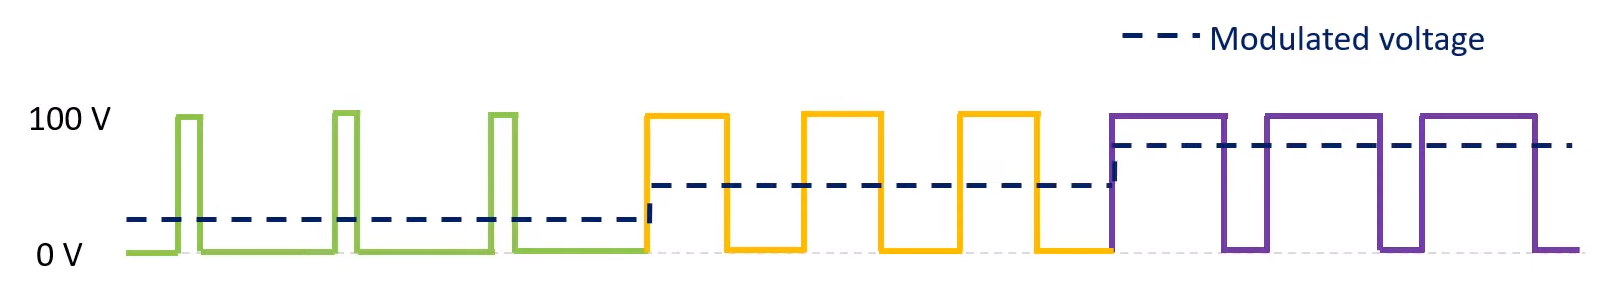
\includegraphics[width=13cm]{imagens/PWM.png} 
     \caption*{Fonte:\cite{matlabBLDC}.} 
  \label{Modulação por largura de pulso utilizando uma fonte de 100V} 
 \end{figure} 

 \subsection{Estratégia de Partida em Malha Aberta para Operação \textit{Sensorless}}

A implementação de um controle \textit{sensorless} eficaz depende da capacidade do controlador de estimar a posição do rotor a partir de grandezas elétricas, mais comumente a FCEM. Contudo, esta abordagem apresenta um desafio fundamental: em repouso (velocidade zero), não há movimento relativo entre os ímãs do rotor e os enrolamentos do estator, e, portanto, nenhuma FCEM é gerada \cite{ti2013sensorless, nxp2023sensorless}. Nesta condição "cega", o controlador não possui informações sobre a posição angular do rotor, tornando impossível determinar qual par de fases deve ser energizado para iniciar a rotação na direção desejada. Para superar essa limitação, é necessária uma rotina de partida especializada, operando em malha aberta, que força o motor a girar até que uma velocidade suficiente seja atingida para que a FCEM se torne detectável e o controle em malha fechada possa assumir. Este procedimento é universalmente dividido em duas fases sequenciais: alinhamento e comutação forçada.

\subsubsection{Alinhamento do Rotor}

O primeiro passo para uma partida confiável é estabelecer uma posição inicial conhecida para o rotor. A fase de alinhamento realiza isso ao energizar um conjunto específico de enrolamentos do estator com uma corrente contínua (DC) por um período de tempo pré-determinado \cite{ti2022minimizing, nxp2023sensorless}. Por exemplo, o controlador pode aplicar uma tensão positiva à fase C e conectar as fases A e B ao terra \cite{ti2022minimizing}. Esta ação cria um campo magnético estático e fixo no estator. Os ímãs permanentes do rotor, livres para girar, irão se alinhar com este campo para minimizar a relutância magnética do circuito, de forma análoga a uma agulha de bússola se alinhando com o campo magnético terrestre. Ao final deste processo, o rotor estará travado em uma posição angular conhecida e previsível. Os parâmetros críticos que governam esta fase são a duração do alinhamento e a magnitude da corrente de alinhamento \cite{ti2022minimizing}.

 A fase de alinhamento funciona como uma etapa de otimização pré-torque, o seu objetivo primordial é condicionar o sistema para que o primeiro passo de comutação dinâmica gere o máximo torque possível. O maior desafio ao iniciar um motor a partir do repouso é vencer a inércia da carga e o atrito estático, o que exige um impulso de torque inicial elevado. A teoria de motores elétricos, conforme estabelecido na Seção 1.1.1, dita que o torque é maximizado quando o campo magnético do estator está orientado a $90^{\circ}$ elétricos em relação ao campo do rotor. O algoritmo de controle é projetado sabendo a posição final do rotor após o alinhamento. Assim, a primeira combinação de fases a ser energizada na fase seguinte (rampa de aceleração) é escolhida para criar um novo vetor de campo magnético do estator que esteja precisamente na orientação ótima em relação à posição agora conhecida do rotor. Isso garante que o primeiro passo dinâmico produza um torque potente e eficaz, "chutando" o rotor para o movimento e superando as resistências iniciais. Uma duração de alinhamento insuficiente ou uma corrente muito baixa pode resultar em um alinhamento incompleto, levando a um torque inicial fraco e, consequentemente, a uma falha na partida \cite{ti2022minimizing, jones2025failures}.

\subsubsection{Comutação Forçada (Rampa de Aceleração)}

Com o rotor devidamente alinhado, o controlador inicia a fase de comutação forçada. Nesta etapa, o sistema opera em malha aberta, comutando as fases em uma sequência predefinida, sem qualquer realimentação da posição do rotor \cite{nxp2023sensorless}. A frequência de comutação não é aplicada abruptamente; em vez disso, ela é aumentada gradualmente a partir de um valor inicial baixo, seguindo um perfil de aceleração pré-programado, conhecido como "curva de partida em malha aberta" (\textit{open-loop starting curve}) \cite{ti2022minimizing}. Esta rampa de aceleração é definida por coeficientes pré-definidos \cite{ti2022minimizing}.

Durante esta fase, o controlador essencialmente comanda a rotação do campo magnético do estator e "assume" que o rotor, devido à sua inércia e ao torque gerado, conseguirá acompanhar este campo giratório. O processo continua, com a frequência de comutação aumentando progressivamente, até que a velocidade de rotação do motor seja alta o suficiente (tipicamente em torno de $5\%$ da velocidade nominal) para que a FCEM gerada nos enrolamentos atinja uma amplitude que possa ser medida de forma confiável \cite{ti2022minimizing, nxp2023sensorless}. Neste ponto, o sistema realiza a transição (\textit{handoff}) do controle em malha aberta para um modo de controle em malha fechada (por exemplo, baseado na detecção de cruzamento por zero da FCEM), que é mais eficiente e robusto para a operação contínua.

\subsection{Desafios e Limitações da Partida Forçada}

Apesar de sua necessidade em sistemas \textit{sensorless}, a estratégia de partida em malha aberta não é isenta de desafios e limitações significativas. A sua natureza "cega" a torna vulnerável a variações de carga e a parâmetros não ideais do sistema.

\subsubsection{Análise do Fenômeno de Perda de Sincronismo (Stall)}

O risco mais proeminente do controle em malha aberta é a perda de sincronismo, comumente conhecida como \textit{stall} ou perda de passo. Este fenômeno ocorre quando a aceleração real do rotor não consegue acompanhar a velocidade de rotação do campo magnético do estator imposta pelo controlador. Se o torque de carga aplicado ao eixo do motor, somado à sua própria inércia, for maior que o torque eletromagnético que o motor consegue produzir em um determinado passo, o rotor "perderá o passo" e ficará para trás \cite{nxp2023sensorless, silva2012controle}. Isso pode ser causado por uma carga inicial muito elevada ou por uma rampa de aceleração excessivamente agressiva, que aumenta a frequência de comutação mais rápido do que o rotor consegue acelerar \cite{ti2022minimizing}.

Uma vez que o sincronismo é perdido, o alinhamento entre os campos do rotor e do estator se torna desfavorável, e a produção de torque efetivo colapsa. O resultado é um movimento errático, vibrações intensas, ruído audível e, frequentemente, a parada completa do motor, enquanto o controlador continua a injetar corrente nos enrolamentos de forma ineficaz. Este estado pode levar a picos de corrente perigosos para a eletrônica de potência. Por essa razão, o controle em malha aberta é inadequado para aplicações com cargas variáveis ou que exigem alto torque de partida.

\subsubsection{Outros Efeitos Adversos}

Além do risco de perda de passo, a partida forçada apresenta outras desvantagens:

\begin{itemize}
    \item \textbf{Picos de Corrente:} No início da partida, a velocidade do motor é baixa ou nula, o que significa que a FCEM — que normalmente se opõe à tensão de alimentação e limita a corrente — também é baixa ou inexistente. Sem essa oposição, a corrente que flui para os enrolamentos é limitada apenas pela resistência ôhmica e pela tensão aplicada, podendo atingir valores muito elevados se não for cuidadosamente controlada pelo \textit{duty cycle} do PWM. Estes picos de corrente podem estressar a bateria e os componentes da ponte inversora.
    \item \textbf{Vibração e Ineficiência:} Como o controle é feito "às cegas", o alinhamento entre o campo do estator e o rotor durante a rampa de aceleração nunca é perfeito. Este desalinhamento constante é a fonte da ondulação de torque discutida anteriormente, que se manifesta como vibração mecânica e resulta em uma operação ineficiente, onde uma parte da energia elétrica consumida é dissipada em vez de ser convertida em torque útil.
\end{itemize}

É fundamental reiterar que a partida forçada em malha aberta é uma fase transitória e um meio para um fim. É uma estratégia de \textit{bootstrap} projetada exclusivamente para levar o motor de um estado de repouso para uma velocidade operacional mínima, onde métodos de controle em malha fechada, mais eficientes, precisos e robustos, podem ser ativados para a operação contínua do sistema \cite{ti2022minimizing, nxp2023sensorless}.

 \subsection{Outros Algoritmos de Controle} 

 Além do Controle Trapezoidal existem outras formas de controle que envolvem algorítimos mais complexos, como o Controle de Torque Vetorial e o Controle de Campo Orientado, ambos em malha fechada. 

 No controle de torque vetorial, o controlador de motor calcula a corrente que deve ser fornecida às bobinas do estator usando um modelo matemático do motor. O modelo matemático do motor descreve a relação entre a corrente nas bobinas do estator, o campo magnético do rotor e o torque produzido pelo motor. O controlador vetorial de torque do motor calcula o torque desejado e, em seguida, usa o modelo matemático do motor para calcular a corrente necessária para produzir o tal torque. Este controle é um método preciso e flexível que pode ser usado em uma variedade de aplicações. Ele é adequado para aplicações onde a exatidão de velocidade e torque é crítica 

 No controle de campo orientado, o controlador do motor calcula a corrente que deve ser fornecida às bobinas do estator usando a orientação do campo magnético do rotor. O controlador de motor usa um sensor para medir a orientação do campo magnético do rotor, sendo que o sensor envia um sinal para o controlador, o utiliza sinal para calcular a corrente necessária para manter o campo magnético do rotor na orientação desejada. O controle de campo orientado é um método preciso e eficiente que pode ser usado em aplicações de alta velocidade. 

 \pagebreak 

 \section{Vantagens e Desvantagens no uso de motores BLDC} 
 Os motores sem escovas, ou BLDC, apresentam diversas vantagens que contribuem para seu destaque em várias aplicações. O rendimento é uma característica proeminente, uma vez que convertem mais eficientemente a energia elétrica em torque quando comparados aos motores com escovas. Isso implica em uma demanda menor de energia para gerar a mesma quantidade de torque, resultando em um melhor desempenho global. A durabilidade é significativamente aprimorada, visto que a vida útil estendida desses motores está relacionada à ausência das escovas, componentes propensos a desgaste em motores convencionais. 

 Os motores de indução trifásicos (MIT) são concorrentes diretos dos motores BLDC, sendo que ambos são amplamente utilizados em diversas aplicações, cada uma com suas características distintas e vantagens específicas. Os motores de indução trifásicos são conhecidos pela sua confiabilidade, simplicidade de construção e custo relativamente baixo, quando comparado aos BLDC, utilizando os princípios da indução eletromagnética para gerar o torque e velocidade necessários para a aplicação. Embora tenham menor custo de produção quando comparados com os motores BLDC e podem ser controlados utilizando os mesmos protocolos, os MITs tendem a ter uma densidade de potência e torque menor em comparação com os motores BLDC, principalmente em baixas velocidades, o que pode ser uma consideração importante em aplicações que requerem alta potência em um espaço limitado. No entanto, os MITs apresentam melhor rendimento em operações de baixo torque, o que pode ser relevante em aplicações de mobilidade, como em veículos elétricos. 

 Os motores BLDC são conhecidos por seu rendimento energético superior, controle preciso de velocidade e torque, além de uma vida útil mais longa devido à ausência de escovas mecânicas \cite{gieras2009permanent}. Embora os BLDCs tenham um custo inicial mais elevado em comparação com os MITs, eles oferecem uma operação mais eficiente, especialmente em condições de carga variável e velocidade ajustável. 

 Em resumo, os motores sem escovas oferecem um conjunto de vantagens notáveis, incluindo rendimento aprimorado, operação mais silenciosa, maior durabilidade e menor necessidade de manutenção. Contudo, esses benefícios vêm com um custo inicial mais elevado e a exigência de um controlador de velocidade, o que pode tornar sua implementação menos acessível em certos contextos. A escolha entre motores com escovas e sem escovas dependerá das prioridades específicas de uma aplicação, considerando tanto os benefícios quanto as limitações de cada tecnologia. 

 \pagebreak 

 \section{Aplicações} 
 Os motores BLDC são amplamente utilizados em diversas aplicações devido às suas características únicas, como elevado rendimento, alta densidade de potência, baixo ruído, baixa manutenção e longa vida útil. Esses motores são preferidos em aplicações que necessitam de controle preciso de torque com oscilações inferiores em comparação com outros motores. 

 Uma das principais aplicações dos motores BLDC é em veículos elétricos, como carros, motocicletas, bicicletas e \textit{scooters} \cite{chau2007emerging}. Com o aumento da demanda por veículos elétricos, espera-se que os motores com tecnologia derivada do BLDC desempenhem um papel vital na indústria automotiva. Esses motores são usados para acionar o sistema de propulsão do veículo, fornecendo torque e potência para as rodas. Eles são preferidos em veículos elétricos devido à seu alta rendimento, baixo ruído e baixa manutenção. Essas motores são usados em aplicações que exigem alta precisão, controle de velocidade e torque, e baixo ruído.

\chapter{Objetivos}
Estudar o princípio de funcionamento de um controlador de motores Brushless, tornando possível o projeto e desenvolvimento de um protótipo que possa oferecer uma operação suave e precisa em diferentes cenários de aplicação.

\chapter{Metodologia}
O desenvolvimento do ESC será realizado seguindo uma abordagem de engenharia de sistemas, partindo da especificação da carga e fonte de energia, passando pelo dimensionamento dos estágios de potência e controle, e finalizando com a validação experimental. A metodologia está estruturada em: definição da arquitetura do sistema, dimensionamento do hardware de potência, desenvolvimento do firmware de controle, simulação computacional e, por fim, a montagem e prototipagem do dispositivo.

\section{Arquitetura do Sistema}
Para a elaboração do projeto físico é necessário o levantamento dos requisitos mínimos que o projeto deve atender, como a categoria de motores e sua fonte de alimentação. A arquitetura proposta consiste em um fluxo de energia que parte de uma bateria de alta descarga, passa por um inversor trifásico controlado, o ESC, e alimenta o motor BLDC. O controle é supervisionado por um microcontrolador que monitora os parâmetros e gera os sinais de modulação.

O projeto do circuito começa pelo levantamento das especificações de carga, seguido pelo dimensionamento da fonte de energia e dos semicondutores de potência. Em paralelo, projeta-se o sistema de controle, definindo o microcontrolador adequado, a lógica de acionamento dos drivers de gate e as estratégias de proteção térmica e de sobrecorrente.

\section{Dimensionamento e Hardware de Potência}
A escolha dos componentes de potência baseia-se nas especificações do motor selecionado, garantindo margens de segurança para operação em regime contínuo e transitório.

\subsection{Especificações do Motor e Carga}
O motor BLDC Turnigy XK3674-$2200KV$ é um modelo comercial projetado principalmente para Automodelismo, sendo do tipo Inrunner possui quatro polos, $2200KV$, Tensão Nominal de $25,2V$, Corrente Nominal de $70A$ e sendo capaz de produzir até $1750W$ de potência. A velocidade e torque a vazio do motor, como já vistos nos segmentos anteriores, é de $55440 RPM$ e $0,3 Nm$, desconsiderando efeitos dissipativos, como o atrito.

\begin{figure}[h]
    \centering
    \caption{Motor Brushless Turnigy XK3674-$2200KV$.}
    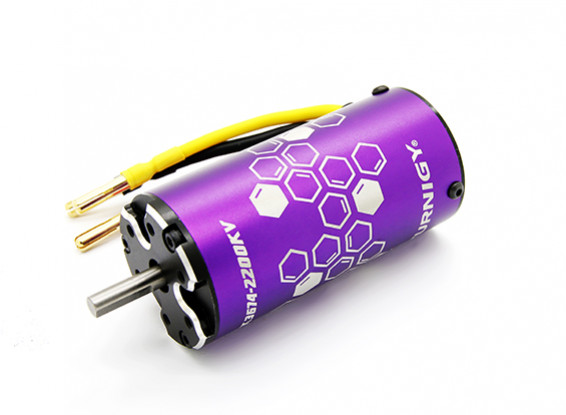
\includegraphics[width=8cm]{imagens/Turnigy XK3674-2200KV.jpg}
    \caption*{Fonte:\cite{turnigyMotor}.}
 \label{Motor Brushless Turnigy XK3674-2200KV}
\end{figure}

\subsection{Fonte de Alimentação Principal (Bateria)}
Em uma aplicação móvel para o ESC devemos fazer uso de baterias como a única fonte de potência para alimentar todo o sistema. Os valores nominais de tensão e corrente do motor a devem ser supridos pela bateria, por volta de $26V$ e $70A$, mas considerando momentos de pico de corrente como por exemplo, uma situação de rotor travado ou de inversão de sentido de rotação é usada uma margem de segurança arbitrária de $30\%$, logo a bateria deve ser capaz de entregar $91A$ de corrente na descarga, um valor considerado alto para baterias.

Atualmente, a tecnologia de bateria com a maior taxa de descarga disponível comercialmente é a bateria de lítio de polímero (LiPo), podendo atingir taxas de descarga muito altas, que podem ultrapassar a $100C$, dependendo da aplicação e do design. 

Baterias LiPo tem três principais características:
\begin{itemize}
\item Tensão Nominal: Diferença de potencial fornecida pela bateria, normalmente é apresentado em em $S$, sendo esse o número de células que a bateira possui, sendo cada célula em média de $3,7V$, logo uma bateria de $7S$ tem uma tensão nominal de $25,9V$; 
\item Capacidade: Indica a quantidade de carga que a bateria pode fornecer antes de ser descarregada completamente, Normalmente é medida em miliampere-horas ($mAh$) ou ampere-horas ($Ah$);
\item Taxa de Descarga (ou \textit{C-rate}): Define a quantidade de corrente que a bateria pode fornecer sem danificar-se, é expressa em múltiplos de $C$.
\end{itemize}

Para calcular a corrente que tais baterias conseguem fornecer podemos aplicar a equação \ref{Corrente de uma bateria LiPo}, desconsiderando efeitos dissipativos ou a variação de tensão nominal que varia de acordo com o nível de carga da bateria, vale ressaltar que a capacidade da bateria deve estar em $Ah$.

\begin{equation}
I = C-rate * Capacidade
\label{Corrente de uma bateria LiPo}
\end{equation}


Uma bateria comercial que atende as especificações do projeto é o modelo Turnigy Graphene Panther $1300mAh$ $6S$ $75C$, capaz de fornecer por volta de $97,5A$, superior a margem de segurança estabelecida. Vale ressaltar que a baterias entrega de tensão nominal $22,2V$, inferior a tensão nominal o que para motores BLDC não é um problema, resultando apenas na redução da  sua velocidade nominal de $55440 RPM$ para $48840RPM$ a vazio, uma redução de aproximadamente $12\%$. 

\begin{figure}[h]
    \centering
    \caption{Turnigy Graphene Panther $1300mAh$ $6S$ $75C$.}
    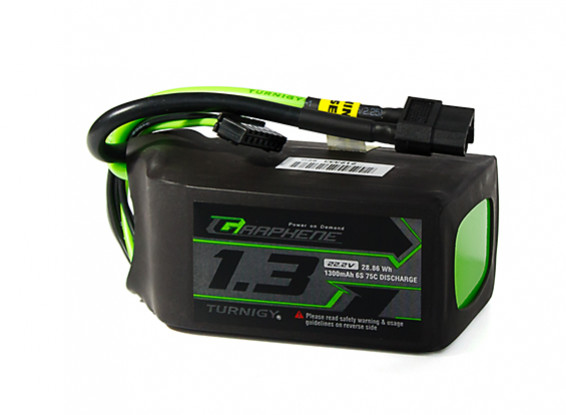
\includegraphics[width=9cm]{imagens/Turnigy Graphene Panther 1300mAh 6S 75C.jpg}
    \caption*{Fonte:\cite{turnigyBattery}.}
 \label{Turnigy Graphene Panther 1300mAh 6S 75C}
\end{figure}

\subsection{Dimensionamento do Inversor (MOSFETs)}
Para o estágio de comutação da ponte inversora trifásica, a escolha do MOSFET foi governada por dois parâmetros críticos: a tensão de ruptura dreno-fonte ($V_{DSS}$), representa o limite máximo de tensão que o dispositivo suporta em seus terminais principais enquanto está em estado de não-condução e a capacidade de dissipação térmica. Considerando que a bateria 6S carregada atinge $25,2V$, e prevendo picos de tensão indutiva ($V_{spike}$) durante o chaveamento, selecionou-se o modelo \textbf{IRFS7530TRL7PP}. Este componente possui um $V_{DSS}$ de $60V$, oferecendo uma margem de segurança superior a 100\% em relação à tensão do barramento DC.

A validação térmica foi realizada considerando a resistência em condução ($R_{DS(on)}$) máxima do componente, que é de aproximadamente $1,4 m\Omega$. Para a corrente de pico projetada de $91A$, a potência dissipada estimada ($P_{diss}$) é dada por:

\begin{equation}
    P_{diss} = I^2 \cdot R_{DS(on)} = 91^2 \cdot 0,0014 \approx 11,6 W
\end{equation}

Embora o encapsulamento D2PAK-7 suporte altas correntes, a dissipação de aproximadamente $11,6W$ exige o uso de uma área de cobre estendida na PCB ou acoplamento com dissipador térmico externo para manter a temperatura de junção dentro dos limites operacionais seguros.

\subsection{Driver de Gate e Circuito de Bootstrap}
O microcontroladores no geral operam com lógica de $3,3V$ ou $5V$, tensão insuficiente para saturar o gate dos MOSFETs de potência, que requerem tipicamente entre $10V$ e $15V$ para garantir a mínima resistência $R_{DS(on)}$. Além disso, o acionamento dos MOSFETs do lado alto (\textit{High-Side}) exige uma tensão flutuante superior à tensão da bateria.

Para solucionar essa interface, foi selecionado o driver de meia-ponte \textbf{IR2110}, capaz de fornecer correntes de pico de até $2A$ para carga e descarga rápida da capacitância de gate ($Q_g$). O driver é alimentado com $15V$ (derivados do circuito BEC), garantindo a saturação completa dos transistores.

Para o acionamento do \textit{High-Side}, utiliza-se a técnica de \textit{Bootstrap}. O capacitor de bootstrap ($C_{boot}$) foi dimensionado para sustentar a carga do gate durante o período de condução. Considerando a carga total de gate do IRFS7530 ($Q_g \approx 360nC$) e as perdas por fuga, optou-se por uma associação em paralelo de um capacitor eletrolítico de $10\mu F$ (reserva de energia) e um cerâmico de $100nF$ (para resposta em alta frequência), garantindo que a queda de tensão no gate seja desprezível mesmo em baixas frequências de comutação.

\subsection{Fonte de Alimentação Auxiliar}
Existem duas abordagens possíveis para a alimentação do microcontrolador e drivers: utilizar uma segunda bateria ou reduzir o nível de tensão da bateria principal. Para otimizar peso e volume, optou-se por um circuito BEC (\textit{Battery Elimination Circuit}).

Dentre as topologias disponíveis, destacam-se os conversores buck (step-down). O conversor Buck é amplamente utilizado para a redução de tensão, operando com elevada eficiência (tipicamente superior a $85\%$) \cite{TIBuckCalculation}. No projeto será aplicado o módulo comercial de baixo custo \textbf{LM2596}, um conversor buck de $150kHz$ e $3A$. O sistema é configurado em cascata: a tensão da bateria ($22,2V - 25,2V$) é regulada para $15V$ para alimentar os drivers IR2110, e subsequentemente reduzida para $5V/3,3V$ para o microcontrolador ESP32.

\begin{figure}[h] 
    \centering 
    \caption{Módulo Comercial LM2596.} 
    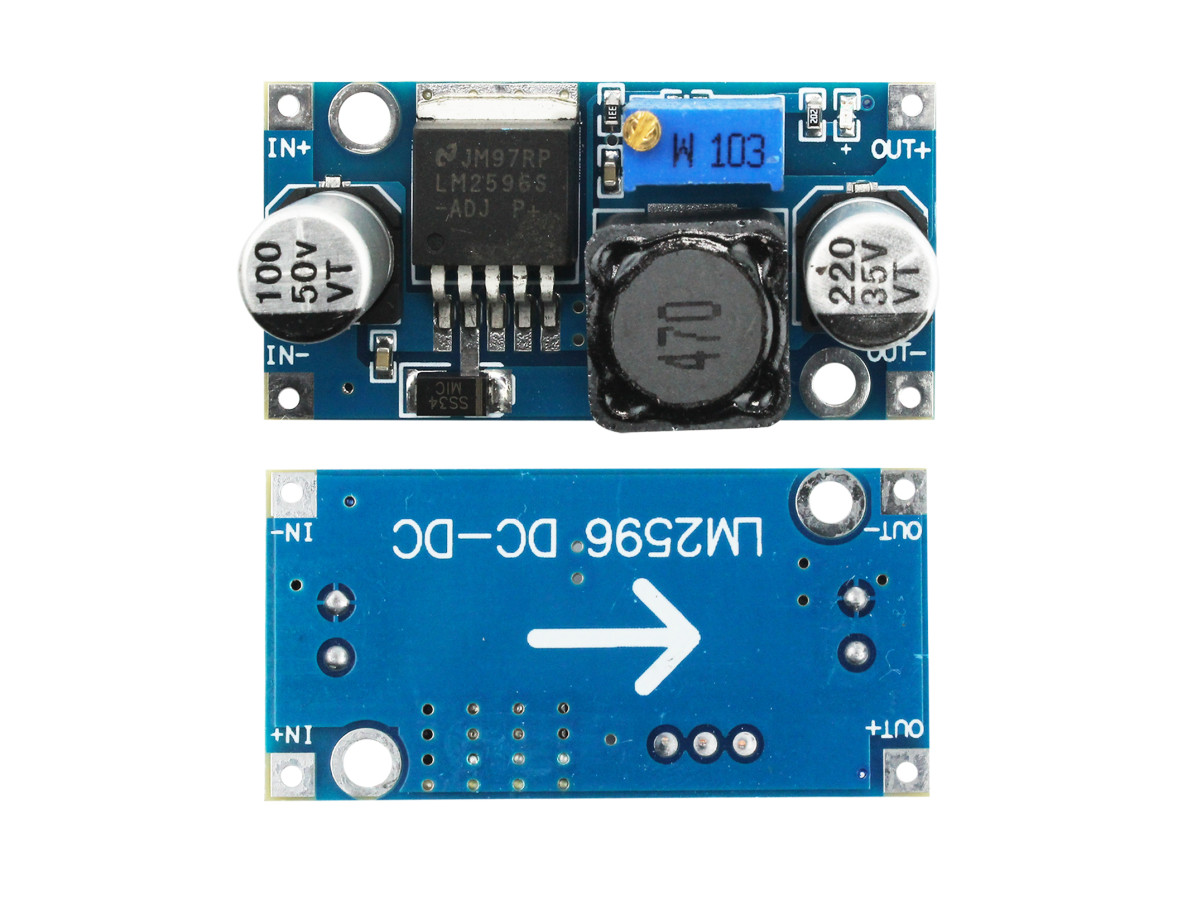
\includegraphics[width=7cm]{imagens/Módulo LM2596.jpg} 
    \caption*{Fonte:\cite{usinaInfoLM2596}.}
\end{figure}

\section{Sistema de Controle e Firmware}
O controle lógico do inversor é centralizado no microcontrolador, responsável pela leitura de sinais, implementação da máquina de estados de comutação e geração dos sinais PWM.

\subsection{O Microcontrolador ESP32}
Para essa aplicação, foi selecionado o ESP32-DevKit C. Utilizando como principal elemento o módulo ESP32-WROOM-32, ele apresenta uma solução robusta para controle em tempo real. Capaz de operar em velocidades de clock de até $240 MHz$, permite a execução paralela de tarefas, característica crítica para sistemas ESC. A resolução de 16 bits dos geradores PWM amplia a precisão no controle da velocidade.

\begin{figure}[H]
    \centering
    \caption{Visão Geral do Microcontrolador ESP32-DevKit C.}
    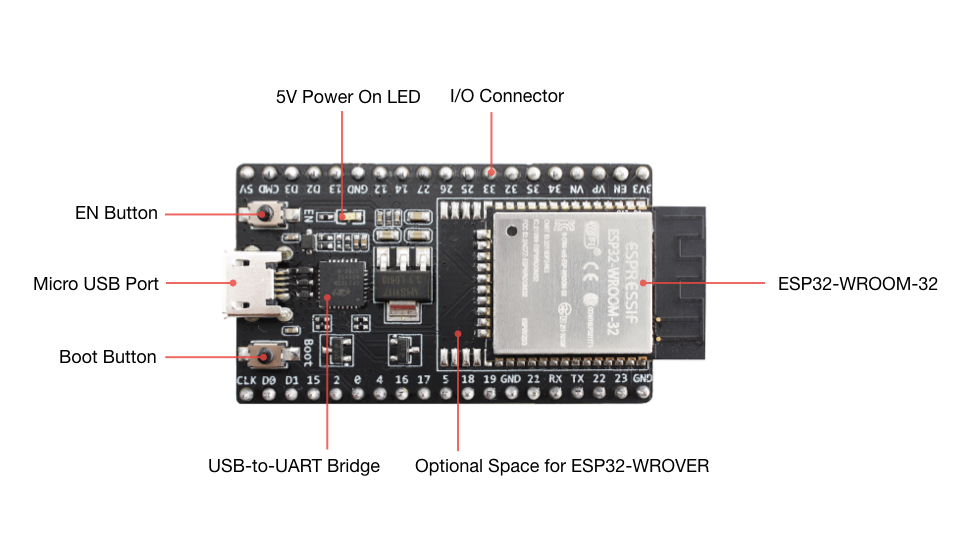
\includegraphics[width=10cm]{imagens/esp32-devkitc-v4-functional-overview.jpg}
    \caption*{Fonte:\cite{ESP32-DevKitCOverview}.}
 \label{esp32DevkitC}
\end{figure}

\begin{figure}[H]
    \centering
    \caption{Pinagem do Microcontrolador ESP32-DevKit C.}
    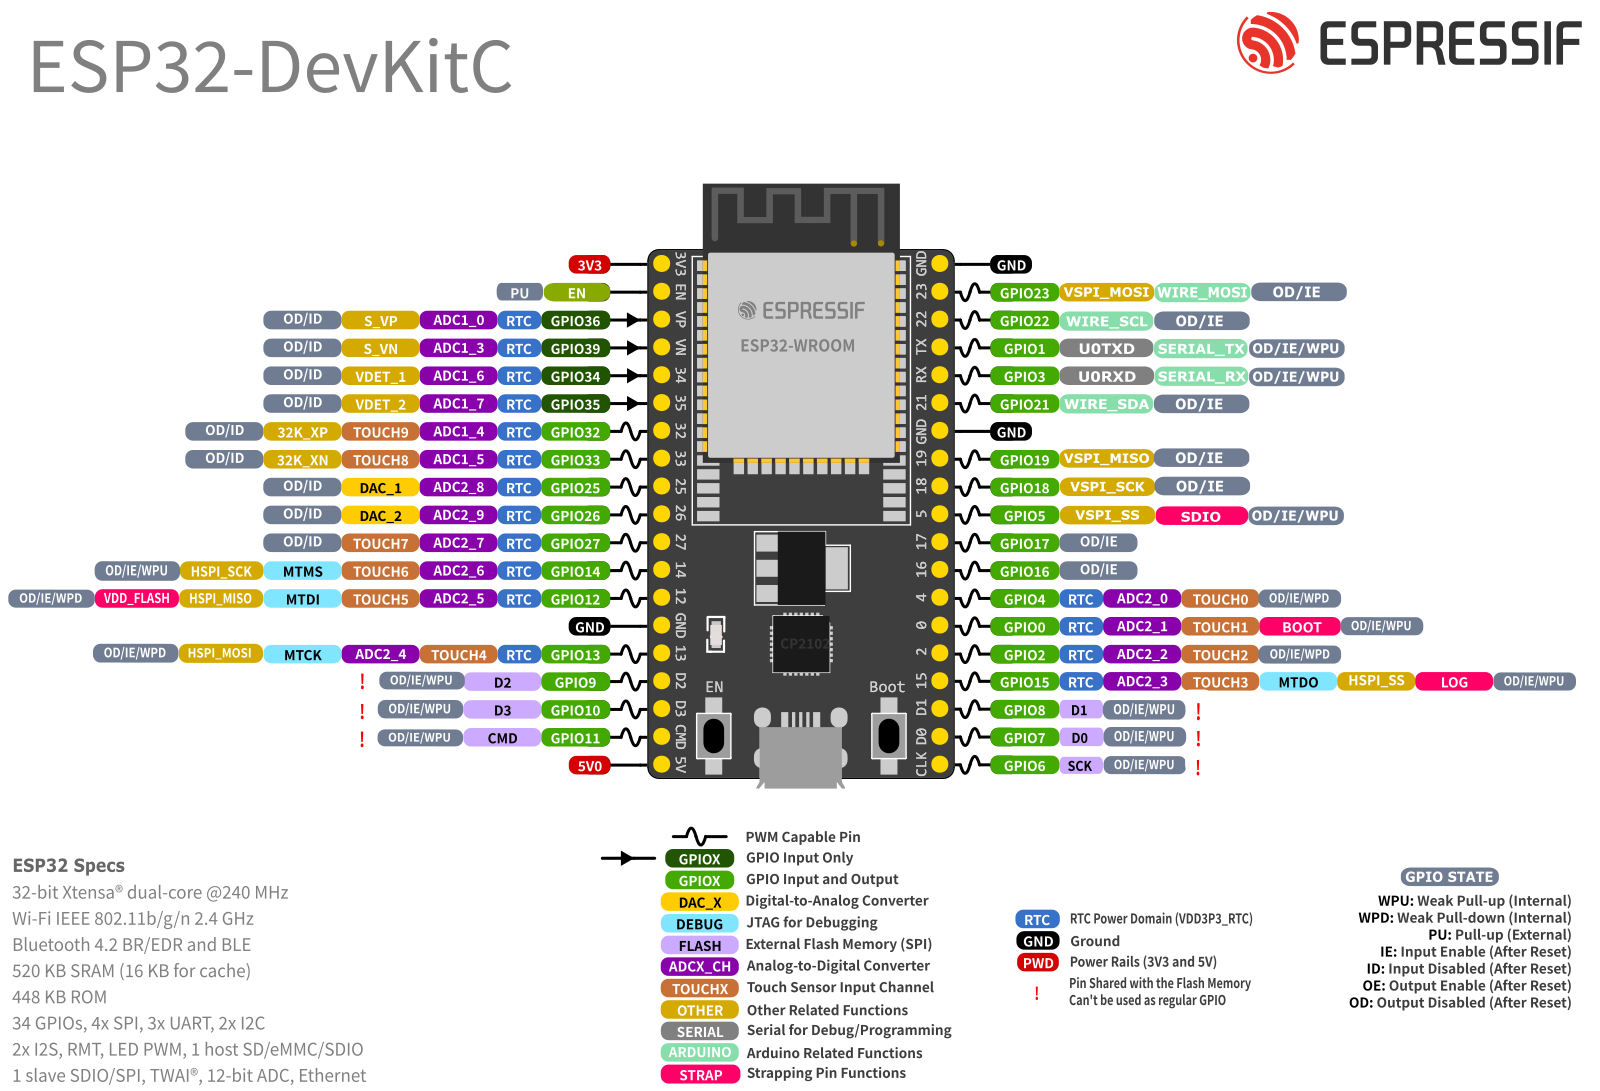
\includegraphics[width=16cm]{imagens/esp32_devkitC_v4_pinlayout.png}
    \caption*{Fonte:\cite{ESP32-DevKitCOverview}.}
 \label{esp32DevkitCPinLayout}
\end{figure}

Apesar dessas vantagens, os níveis lógicos de $3,3V$ exigiram o uso dos drivers IR2110 mencionados anteriormente para a interface com a potência.

\subsection{Lógica de Comutação de Seis Passos}
A lógica de chaveamento constitui o núcleo funcional do ESC. Nesta abordagem, utiliza-se a comutação de seis passos em malha aberta (\textit{Sensorless}). A ponte inversora trifásica é acionada de forma que apenas dois MOSFETs conduzam simultaneamente a cada passo, criando um campo magnético giratório que avança em incrementos de $60^{\circ}$.

\begin{table}[H]
    \centering
    \caption{Sequência de Comutação de Seis Passos e Estado dos MOSFETs}
    \label{tab:logica_seis_passos}
    \begin{tabular}{@{}cccccccc@{}} 
        \toprule
        \textbf{Passo} & \textbf{Pos. Elétrica} & \textbf{High A} & \textbf{Low B} & \textbf{High C} & \textbf{Low A} & \textbf{High B} & \textbf{Low C} \\ \midrule
        1 & 0° -- 60°   & ON & ON  & OFF & OFF & OFF & OFF \\
        2 & 60° -- 120°  & ON & OFF & OFF & OFF & OFF & ON  \\
        3 & 120° -- 180° & OFF& OFF & ON  & OFF & ON  & OFF \\
        4 & 180° -- 240° & OFF& OFF & ON  & ON  & OFF & OFF \\
        5 & 240° -- 300° & OFF& ON  & OFF & ON  & OFF & OFF \\
        6 & 300° -- 360° & OFF& OFF & OFF & OFF & ON  & ON  \\ \bottomrule
    \end{tabular}
    \caption*{Fonte: Elaborado pelo autor.}
\end{table}

\subsection{Implementação Prática com o Periférico MCPWM}
A implementação da comutação no firmware utiliza o periférico dedicado \textit{Motor Control Pulse Width Modulator} (MCPWM) do ESP32 \cite{esp32-technical-reference-manual}. Este módulo desonera a CPU da geração de sinais e insere automaticamente o tempo morto (\textit{Dead Time}) necessário para evitar curto-circuitos na ponte H (shoot-through).

A configuração segue o mapeamento da Tabela \ref{tab:mcpwm_map}, onde o \textit{Duty Cycle} é aplicado ao transistor do lado alto (High-Side) para controle de corrente, enquanto o lado baixo (Low-Side) é mantido em condução plena ou chaveado de forma complementar, dependendo da estratégia de frenagem regenerativa desejada.

\begin{table}[H]
    \centering
    \caption{Mapeamento dos Estados de Comutação para os Geradores MCPWM do ESP32}
    \label{tab:mcpwm_map}
    \resizebox{\textwidth}{!}{%
        \begin{tabular}{@{}ccccccc@{}}
            \toprule
            \textbf{Passo} & \textbf{Fases Energizadas} & \textbf{High-Side} & \textbf{Low-Side} & \textbf{OPR 0 (A)} & \textbf{OPR 1 (B)} & \textbf{OPR 2 (C)} \\ \midrule
            1 & A+ B- & T1 & T4 & PWM / LOW & LOW / ACTIVE & Hi-Z / Hi-Z \\
            2 & A+ C- & T1 & T6 & PWM / LOW & Hi-Z / Hi-Z & LOW / ACTIVE \\
            3 & B+ C- & T3 & T6 & Hi-Z / Hi-Z & PWM / LOW & LOW / ACTIVE \\
            4 & B+ A- & T3 & T2 & LOW / ACTIVE & PWM / LOW & Hi-Z / Hi-Z \\
            5 & C+ A- & T5 & T2 & LOW / ACTIVE & Hi-Z / Hi-Z & PWM / LOW \\
            6 & C+ B- & T5 & T4 & Hi-Z / Hi-Z & LOW / ACTIVE & PWM / LOW \\ \bottomrule
        \end{tabular}
    }
    \flushleft
    \footnotesize{\textit{Nota:} "PWM / LOW" indica modulação. "LOW / ACTIVE" indica condução ao terra. "Hi-Z" alta impedância.} 
\end{table}

\subsection{Estratégia de Partida (Malha Aberta)}
Dado que o controle \textit{Sensorless} não possui informação de posição em velocidade zero, implementa-se uma rotina de partida em duas etapas. Primeiramente, a fase de \textbf{Alinhamento}, onde uma tensão fixa é aplicada a um par de fases específico por um tempo determinado (ex: 500ms), forçando o rotor a uma posição conhecida. Em seguida, inicia-se a \textbf{Rampa de Aceleração}, onde a frequência de comutação entre os estados da Tabela \ref{tab:logica_seis_passos} é incrementada gradualmente em malha aberta até que o motor atinja velocidade suficiente para estabilização mecânica.

\section{Simulação Computacional}
Para validar a lógica de controle e a integridade dos sinais de disparo antes da montagem física, utiliza-se a simulação computacional. Devido à complexidade dos modelos SPICE proprietários para os drivers de gate, opta-se pelo uso de modelos comportamentais equivalentes em software de simulação de circuitos (ex: LTSpice ou Proteus). A simulação foca na verificação das formas de onda de tensão de linha e de fase, bem como na garantia de que a sequência de seis passos não gera sobreposição de condução nos braços do inversor.

\section{Montagem e Prototipagem}
A etapa final consiste na integração física dos subsistemas. O controlador é montado em uma placa de circuito impresso (PCB) desenhada para suportar as altas correntes do barramento DC, com trilhas reforçadas e planos de terra adequados. O microcontrolador é programado com a lógica desenvolvida e o sistema é submetido a testes de bancada, iniciando com cargas leves e alimentação limitada para verificação de segurança (teste de fumaça), progredindo para o acionamento do motor em rampa de velocidade para validação do protótipo funcional.

Todas as etapas de validação e os resultados obtidos, tanto na simulação quanto nos ensaios práticos, são documentados no capítulo subsequente de Resultados.

% --- ELEMENTOS PÓS-TEXTUAIS ---
\postextual
\printbibliography

\end{document}